\documentclass[border=8pt]{standalone}
\usepackage[scaled]{helvet}
\renewcommand\familydefault{\sfdefault}
\usepackage{tikz}
\usetikzlibrary{arrows.meta, positioning, fit, calc}

\definecolor{inGray}{HTML}{F0F0F0}
\definecolor{proc}{HTML}{ECECFF}
\definecolor{core}{HTML}{FDEBD9}
\definecolor{outGreen}{HTML}{E2FBE2}

\tikzset{
  box/.style={draw, rounded corners=3pt, align=center, minimum height=1.1cm,
              font=\small, inner sep=4pt},
  inbox/.style={box, fill=inGray, minimum width=2.9cm},
  procbox/.style={box, fill=proc, minimum width=2.9cm},
  outbox/.style={box, fill=outGreen, minimum width=2.9cm},
  arr/.style={-{Stealth[length=2.2mm]}, semithick},
  darr/.style={arr, dashed},
}

\begin{document}
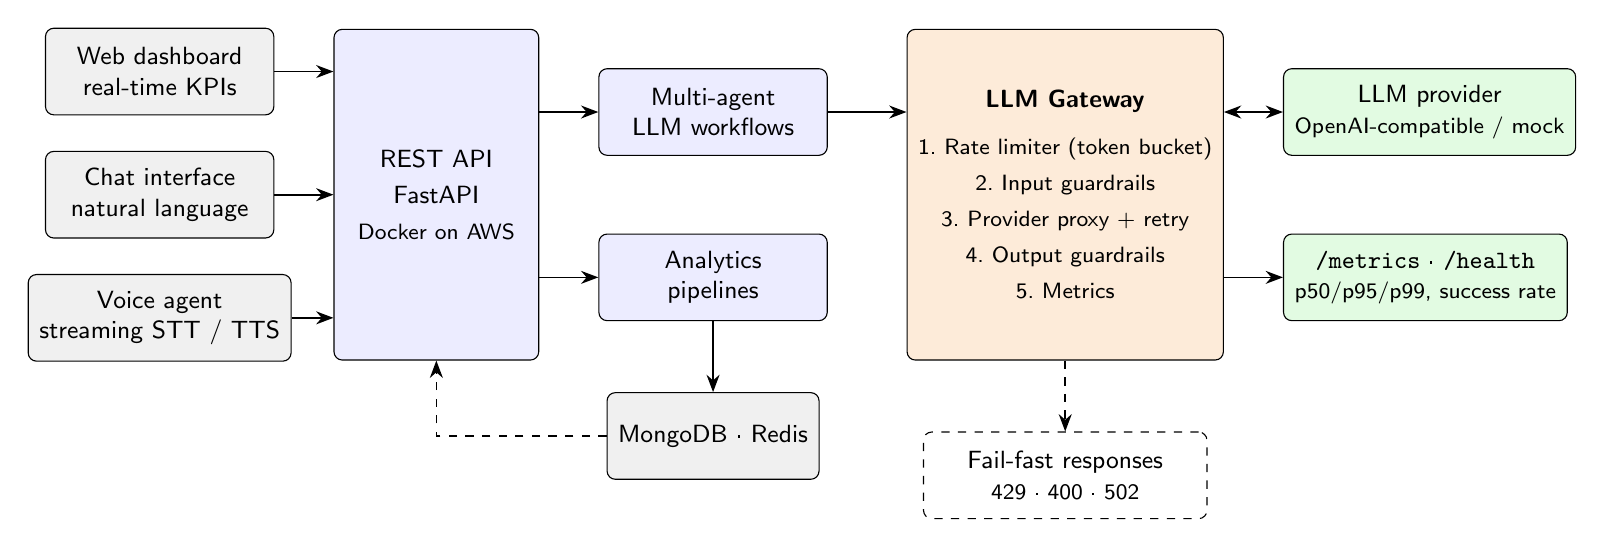
\begin{tikzpicture}[node distance=0.45cm and 0.75cm]

% --- clients ---
\node[inbox] (web)  {Web dashboard\\real-time KPIs};
\node[inbox, below=of web] (chat) {Chat interface\\natural language};
\node[inbox, below=of chat] (voice) {Voice agent\\streaming STT / TTS};

% --- api ---
\node[procbox, right=of chat, minimum height=4.2cm, minimum width=2.6cm] (api)
  {REST API\\[2pt]FastAPI\\[2pt]\footnotesize Docker on AWS};

% --- workflows ---
\node[procbox, right=of api, yshift=1.05cm] (agents) {Multi-agent\\LLM workflows};
\node[procbox, right=of api, yshift=-1.05cm] (pipes) {Analytics\\pipelines};

% --- gateway ---
\node[box, fill=core, right=1.0cm of agents, yshift=-1.05cm,
      minimum width=3.6cm, minimum height=4.2cm] (gw)
  {\textbf{LLM Gateway}\\[6pt]
   \footnotesize 1.\ Rate limiter (token bucket)\\[2pt]
   \footnotesize 2.\ Input guardrails\\[2pt]
   \footnotesize 3.\ Provider proxy + retry\\[2pt]
   \footnotesize 4.\ Output guardrails\\[2pt]
   \footnotesize 5.\ Metrics};

% --- provider + outputs ---
\node[outbox, right=of gw, yshift=1.05cm] (llm) {LLM provider\\\footnotesize OpenAI-compatible / mock};
\node[outbox, right=of gw, yshift=-1.05cm] (obs) {\texttt{/metrics} \textperiodcentered{} \texttt{/health}\\\footnotesize p50/p95/p99, success rate};

% --- data + fail-fast ---
\node[inbox, below=0.9cm of pipes, minimum width=2.6cm] (db) {MongoDB \textperiodcentered{} Redis};
\node[box, dashed, below=0.9cm of gw, minimum width=3.6cm] (err)
  {Fail-fast responses\\\footnotesize 429 \textperiodcentered{} 400 \textperiodcentered{} 502};

% --- edges ---
\draw[arr] (web.east)   -- (web.east -| api.west);
\draw[arr] (chat.east)  -- (api.west);
\draw[arr] (voice.east) -- (voice.east -| api.west);

\draw[arr] (api.east |- agents.west) -- (agents.west);
\draw[arr] (api.east |- pipes.west)  -- (pipes.west);
\draw[arr] (agents.east) -- (agents.east -| gw.west);

\draw[arr, {Stealth[length=2.2mm]}-{Stealth[length=2.2mm]}] (gw.east |- llm.west) -- (llm.west);
\draw[arr] (gw.east |- obs.west) -- (obs.west);
\draw[darr] (gw.south) -- (err.north);

\draw[arr] (pipes.south) -- (db.north);
\draw[darr] (db.west) -| (api.south);

\end{tikzpicture}
\end{document}
